\chapter{字符串}
\label{字符串}


\section{字符串是一个序列}
\index{序列}
\index{字符}
\index{括号运算符}
\index{运算符!括号}

字符串是字符的 {\bf 序列} 。你可以使用括号运算符每次访问一个字符。 

\beforeverb
\begin{verbatim}
>>> fruit = 'banana'
>>> letter = fruit[1]
\end{verbatim}
\afterverb
%
第二条语句从{\tt fruit}中读取第一个字符,并赋值给{\tt letter}。

\index{下标}

在括号中的表达式称为{\bf 下标}。下标指示了序列中对应的字符。

但是你也许没有得到你期望的:

\beforeverb
\begin{verbatim}
>>> print letter
a
\end{verbatim}
\afterverb
%
对于大多数人来说,\verb"'banana'"是{\tt b},而不是{\tt a}。但是对计算机科学家来说,下标是从字符串开始位置的偏移量,第一个字符的偏移量是零。

\beforeverb
\begin{verbatim}
>>> letter = fruit[0]
>>> print letter
b
\end{verbatim}
\afterverb
%
所以{\tt b}是\verb"'banana'"中第零个字符,{\tt a}是第一个字符,{\tt n}是第二个字符。

\index{下标!从零开始}
\index{零,下标开始}

你可以使用包含变量和运算符的表达式作为下标,但下标值必须是一个整数,否则你将得到:

\index{下标}
\index{异常!类型错误}
\index{类型错误}

\beforeverb
\begin{verbatim}
>>> letter = fruit[1.5]
TypeError: string indices must be integers
\end{verbatim}
\afterverb
%

\section{{\tt len}}

\index{len函数}
\index{函数!len}

{\tt len}是一个内建函数,返回一个字符串的长度:

\beforeverb
\begin{verbatim}
>>> fruit = 'banana'
>>> len(fruit)
6
\end{verbatim}
\afterverb
%
要得到一个字符串最有一个字符,你可以这么做:

\index{异常!下标错误}
\index{下标错误}

\beforeverb
\begin{verbatim}
>>> length = len(fruit)
>>> last = fruit[length]
IndexError: string index out of range
\end{verbatim}
\afterverb
%
{\tt 下表错误}的原因是因为{\tt 'banana'}中没有字符下标为6。下标从0开始计数,6个字符的下标分别是0到5。要得到最后一个字符,你要对{\tt length}减1:

\beforeverb
\begin{verbatim}
>>> last = fruit[length-1]
>>> print last
a
\end{verbatim}
\afterverb
%
另一个方式是使用负数下标,它将从字符串尾部计数。表达式{\tt fruit[-1]}返回最后一个字符,{\tt fruit[-2]}返回倒数第二个字符,以此类推。

\index{下标!负数}
\index{负数下标}


\section{使用{\tt for}循环遍历}
\label{for}

\index{遍历}
\index{循环!遍历}
\index{for循环}
\index{循环!for}
\index{语句!for}
\index{遍历}

许多计算包含对字符串字母逐一操作。通常从字符串头开始,每次选择一个字符进行操作,直到字符串尾。这个过程称为{\bf 遍历}。遍历的一个方法是使用{\tt while}循环:

\beforeverb
\begin{verbatim}
index = 0
while index < len(fruit):
    letter = fruit[index]
    print letter
    index = index + 1
\end{verbatim}
\afterverb
%
这个循环遍历字符串并在每行打印一个字母。循环条件是{\tt index < len(fruit)},当{\tt index}等于字符串的长度,条件为假,循环的主体将不再执行。最后一个被访问的字符的下标是{\tt len(fruit)-1},对应字符串的最后一个字符。

\begin{ex}
编写一个函数,读取一个字符串作为参数,逆序打印字符串,每行一个字符。
\end{ex}

遍历的另一个方法是使用{\tt for}循环:

\beforeverb
\begin{verbatim}
for char in fruit:
    print char
\end{verbatim}
\afterverb
%
对于每一次循环,字符串中的下一个字符被赋值给变量{\tt char}。当所有字符都赋值过后,循环结束。

\index{连接}
\index{字母表}
\index{McCloskey, Robert}

下面的例子演示了如何使用连接(字符串相加)和{\tt for}循环来生成一个字母表(即字母顺序)。在Robert McCloskey的{\em Make Way for Ducklings}中,小鸭子们的名字为Jack, Kack, Lack,Mack, Nack, Ouack, Pack和Quack。

\beforeverb
\begin{verbatim}
prefixes = 'JKLMNOPQ'
suffix = 'ack'

for letter in prefixes:
    print letter + suffix
\end{verbatim}
\afterverb
%
输出为:

\beforeverb
\begin{verbatim}
Jack
Kack
Lack
Mack
Nack
Oack
Pack
Qack
\end{verbatim}
\afterverb
%
当然这不完全正确,因为”Ouack“和”Quack“拼写错误了。

\begin{ex}
修改程序以修复错误。
\end{ex}



\section{字符串切片}
\label{切片}

\index{切片运算符}
\index{运算符!切片}
\index{下标!切片}
\index{字符串!切片}
\index{切片!字符串}

字符串的一段称为{\bf 切片}。选择字符串的一个切片和选择一个字符类似:

\beforeverb
\begin{verbatim}
>>> s = 'Monty Python'
>>> print s[0:5]
Monty
>>> print s[6:12]
Python
\end{verbatim}
\afterverb
%
运算符{\tt [n:m]}返回字符串中第n到第m个字符,包括第n个字符,但不包括第m个字符。这种行为是违反直觉的,但是我们可以通过想象在在字符间放置标号来帮助理解,如下图所示:

\beforefig
\centerline{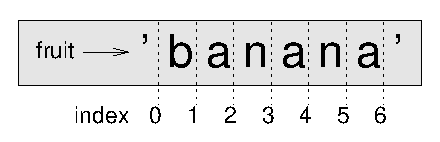
\includegraphics{figs/banana.eps}}
\afterfig

如果你忽略第一个下标(在冒号之前),切片开始于字符串的头部。如果你忽略第二个下标,切片将结束于字符串的尾部:

\beforeverb
\begin{verbatim}
>>> fruit = 'banana'
>>> fruit[:3]
'ban'
>>> fruit[3:]
'ana'
\end{verbatim}
\afterverb
%
如果第一个下标大于等于第二个下标,结果将为一个{\bf 空字符串},用两个引号表示:

\index{引号标记}

\beforeverb
\begin{verbatim}
>>> fruit = 'banana'
>>> fruit[3:3]
''
\end{verbatim}
\afterverb
%
空字符串不包含任何字符且长度为零,除此以外和其他字符串相同。

\begin{ex}
假设{\tt fruit}是一个字符串,{\tt fruit[:]}是什么?

\index{复制!切片}
\index{切片!复制}

\end{ex}


\section{字符串是不变的}
\index{可变}
\index{不可变}
\index{字符串!不可变}

下面尝试使用{\tt []}运算符作为赋值语句的左值,试图改变字符串中的字符:

\index{类型错误}
\index{异常!类型错误}

\beforeverb
\begin{verbatim}
>>> greeting = 'Hello, world!'
>>> greeting[0] = 'J'
TypeError: object does not support item assignment
\end{verbatim}
\afterverb
%
在本例中”对象“是字符串,”项目“是你试图赋值的字符。现在,一个”对象“等同于一个数值,以后我们会重新进行定义。一个”项目“是序列中的一个值。

\index{对象}
\index{项目赋值}
\index{赋值!项目}
\index{不可变}

错误的原因是因为字符串是{\bf 不可变的},即你不可以修改一个已经存在的字符串。你可以做的是新建一个字符串并在原来的基础上修改:

\beforeverb
\begin{verbatim}
>>> greeting = 'Hello, world!'
>>> new_greeting = 'J' + greeting[1:]
>>> print new_greeting
Jello, world!
\end{verbatim}
\afterverb
%
例子中将新的第一个字母和{\tt greeting}的一个切片连接,这个操作对原来字符串没有影响。

\index{连接}


\section{搜索}
\label{查找}

以下函数实现了什么功能?

\index{find函数}
\index{函数!find}

\beforeverb
\begin{verbatim}
def find(word, letter):
    index = 0
    while index < len(word):
        if word[index] == letter:
            return index
        index = index + 1
    return -1
\end{verbatim}
\afterverb
%
从某种角度来说,{\tt find}是{\tt []}运算符的反操作。它读取字符,寻找字符串中对应的下标。如果字符没有找到,函数返回{\tt -1}。

这是我们看到的第一个{\tt return}语句在循环体中的例子。如果{\tt word[index] == letter},函数中断跳出循环,并立即返回。

如果字符串中不存在该字符,程序正常退出循环并返回{\tt -1}。

这种遍历序列寻找我们需要的内容的计算模式称为{\bf 搜索}。

\index{遍历}
\index{搜索模式}
\index{模式!搜索}

\begin{ex}
修改{\tt find}函数,增加第三个参数{\tt word},指示开始搜索的位置。
\end{ex}


\section{循环和记数}
\label{记数}

\index{记数}
\index{记数和循环}
\index{循环和记数}
\index{循环!关于字符串}

下面的程序统计字符{\tt a}在字符串中出现的次数:

\beforeverb
\begin{verbatim}
word = 'banana'
count = 0
for letter in word:
    if letter == 'a':
        count = count + 1
print count
\end{verbatim}
\afterverb
%
程序演示了另一种计算模式{\bf 记数}。变量{\tt count}首先被初始化为0,然后每次发现{\tt a}就增加1。当循环退出后,{\tt count}记录了{\tt a}总共出现的次数。

\begin{ex}
\index{封装}

将代码封装成一个名叫{\tt count}的函数,推广函数是得它可以接收字符串和字符作为参数。

\end{ex}

\begin{ex}
重写函数,使用3个参数的{\tt find}版本,而不是遍历字符串。
\end{ex}


\section{{\tt string}方法}

{\bf 方法}类似函数,它读取参数,并返回一个值,但两者语法有区别。例如,方法{\tt upper}读取一个字符串并返回一个全大写的新字符串:

\index{方法}
\index{字符串!方法}

相比函数的语法{\tt upper(word)},方法的语法为{\tt word.upper()}。

\index{点符号}

\beforeverb
\begin{verbatim}
>>> word = 'banana'
>>> new_word = word.upper()
>>> print new_word
BANANA
\end{verbatim}
\afterverb
%
这样的点符号的形式指定了方法的名称{\tt upper},以及方法作用的字符串名{\tt word}。空的括号指示这个方法不读取参数。

\index{括号!空}

一个方法的调用称为{\bf 调用};在本例中,我们称对{\tt word}调用了{\tt upper}方法。

\index{调用}

事实上,字符串有一个方法{\tt find}十分类似我们写的函数:

\beforeverb
\begin{verbatim}
>>> word = 'banana'
>>> index = word.find('a')
>>> print index
1
\end{verbatim}
\afterverb
%
在这个例子中,我们对{\tt word}调用了{\tt find}方法,并传入我们需要寻找的字符作为参数。

事实上,{\tt find}方法比我们的函数适用更广,它不仅可以查找字符,也可以查找子串:

\beforeverb
\begin{verbatim}
>>> word.find('na')
2
\end{verbatim}
\afterverb
%
它可以读取第二个参数来指定开始查找的位置:

\index{可选参数}
\index{参数!可选}

\beforeverb
\begin{verbatim}
>>> word.find('na', 3)
4
\end{verbatim}
\afterverb
%
还有第三个参数,指定查找结束的位置:

\beforeverb
\begin{verbatim}
>>> name = 'bob'
>>> name.find('b', 1, 2)
-1
\end{verbatim}
\afterverb
%
这次查找失败,因为{\tt b}在查找范围{\tt 1}到{\tt 2}中不存在(不包含{\tt 2})。


\begin{ex}
\index{记数方法}
\index{方法!记数}

字符串有个方法称为{\tt count},类似先前练习中的函数。阅读这个方法的文档,编写方法调用,统计{\tt a}在\verb"'banana'"中出现的次数。
\end{ex}


\section{{\tt in}运算符}
\label{inboth}

\index{in运算符}
\index{运算符!in}
\index{布尔运算符}
\index{运算符!布尔}

{\tt in}是一个布尔运算符,它读取两个字符串作为参数,如果第一个字符串是第二个字符串的子串,则返回{\tt True}:

\beforeverb
\begin{verbatim}
>>> 'a' in 'banana'
True
>>> 'seed' in 'banana'
False
\end{verbatim}
\afterverb
%
例如,下面的函数打印在{\tt word1}和{\tt word2}中同时出现的字符:

\beforeverb
\begin{verbatim}
def in_both(word1, word2):
    for letter in word1:
        if letter in word2:
            print letter
\end{verbatim}
\afterverb
%
如果函数名是精心挑选的,Python有时读起来想英语。你可以这么读一个循环:“for (each) letter in (the first) word, if (the) letter (appears) in (the second) word, print (the) letter.”

下面是你比较apples和oranges的输出:

\beforeverb
\begin{verbatim}
>>> in_both('apples', 'oranges')
a
e
s
\end{verbatim}
\afterverb
%

\section{字符串比较}

\index{字符串!比较}
\index{比较!字符串}

关系运算符可以作用在字符串上。看两个字符串是否相等:

\beforeverb
\begin{verbatim}
if word == 'banana':
    print  'All right, bananas.'
\end{verbatim}
\afterverb
%
其他关系运算符可以用来将单词按字母表排序:

\beforeverb
\begin{verbatim}
if word < 'banana':
    print 'Your word,' + word + ', comes before banana.'
elif word > 'banana':
    print 'Your word,' + word + ', comes after banana.'
else:
    print 'All right, bananas.'
\end{verbatim}
\afterverb
%
Python不像人们一样处理大小写字母。所有的大写字母在小写字母之前,所以:

\beforeverb
\begin{verbatim}
Your word, Pineapple, comes before banana.
\end{verbatim}
\afterverb
%
一个常用的解决这个问题的方法是在比较前将字符串转化为一个标准的格式,如全小写。


\section{调试}
\index{调试}

\index{遍历}
当使用下标遍历序列的值时,很容易将遍历的开始位置和结束位置搞错。这里给出了一个函数,它试图比较两个单词,如果一个是另一个的逆序则返回{\tt True},函数中有两个错误:

\beforeverb
\begin{verbatim}
def is_reverse(word1, word2):
    if len(word1) != len(word2):
        return False
    
    i = 0
    j = len(word2)

    while j > 0:
        if word1[i] != word2[j]:
            return False
        i = i+1
        j = j-1

    return True
\end{verbatim}
\afterverb
%
第一个{\tt if}语句检查两个单词是否长度相同。如果不相同,我们可以立即返回{\tt False}。否则,我们可以保证两个单词长度相同。这是章节~\ref{守护人}中一个守护人模式的例子。

\index{守护人模式}
\index{模式!守护人}
\index{下标}

{\tt i}和{\tt j}是下标,{\tt i}从前往后遍历{\tt word1},而{\tt j}从后往前遍历{\tt word2}。如果我们发现两个字符不同,我们可以立即返回{\tt False}。如果我们完成整个循环,即所有字符都匹配,我们返回{\tt True}。

如果我们用“pots”和“stop”来测试这个函数,我们期望返回值为{\tt True},然而我们得到下标错误:

\index{下标错误}
\index{异常!下标错误}

\beforeverb
\begin{verbatim}
>>> is_reverse('pots', 'stop')
...
  File "reverse.py", line 15, in is_reverse
    if word1[i] != word2[j]:
IndexError: string index out of range
\end{verbatim}
\afterverb
%
为了调试这类错误,我第一步是在错误的行前面打印相应的值:

\beforeverb
\begin{verbatim}
    while j > 0:
        print i, j        # print here
        
        if word1[i] != word2[j]:
            return False
        i = i+1
        j = j-1
\end{verbatim}
\afterverb
%
现在再次运行程序,我得到更多的信息:

\beforeverb
\begin{verbatim}
>>> is_reverse('pots', 'stop')
0 4
...
IndexError: string index out of range
\end{verbatim}
\afterverb
%
在第一次穿越循环后,{\tt j}的值是4,超过了\verb"'pots'"的长度。最后一个字符对应的下标是3,所以{\tt j}的初始值应该为{\tt len(word2)-1}。

\index{语义错误}
\index{错误!语义}

我修正了这个错误,再次运行程序得到:

\beforeverb
\begin{verbatim}
>>> is_reverse('pots', 'stop')
0 3
1 2
2 1
True
\end{verbatim}
\afterverb
%
这次我们得到正确的结果,但看起来循环只运行了3次,十分可疑。为了弄清楚是怎么回事,一个很有效的方法是画状态图。在第一次迭代中,\verb"is_reverse"的第一帧如下:

\index{状态图}
\index{图!状态}

\beforefig
\centerline{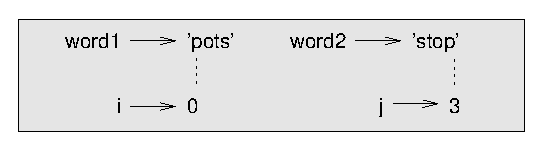
\includegraphics{figs/state4.eps}}
\afterfig

我用虚线标记出变量{\tt i}和{\tt j}对应{\tt word1}和{\tt word2}中的字符。

\begin{ex}
\label{is_reverse}
从这个图开始,在纸上运行程序,在每次迭代中修改{\tt i}和{\tt j}的值。找出并修改函数中的错误。
\end{ex}



\section{术语}

\begin{description}

\item[对象:] 变量可以指向的东西。到目前,你可以互换的使用“对象”和“值”。
\index{对象}

\item[序列:] 一个有序的集合,每一个集合中的数对应一个整数下标。
\index{序列}

\item[项目:] 序列中的一个项目。
\index{项目}

\item[下标:] 序列中用于选择项目的一个整数值,如字符串中的一个字符。
\index{下标}

\item[切片:] 有一定下标确定的字符串的一部分。
\index{切片}

\item[空字符串:] 一个没有字符的长度为0的字符串,使用两个引号表示。
\index{空字符串}

\item[不可变:] 序列中的项目不可改变的性质。
\index{不可变}

\item[遍历:] 迭代访问序列中的每个项目,并执行类似的操作。
\index{遍历}

\item[查找:] 遍历的一种模式,当找到要找的内容时停止。
\index{查找模式}
\index{模式!查找}

\item[计数器:] 用来计数的变量,通常初始化为0,然后递增。
\index{计数器}

\item[方法:] 一个和对象关联的函数,应用点符号来调用。
\index{方法}

\item[调用:] 调用方法的语句。
\index{调用}

\end{description}


\section{练习}

\begin{ex}

\index{步长}
\index{切片运算符}
\index{运算符!切片}

字符串的切片可以读取第三个参数“步长”,它决定了相邻字符之间的间隔。步长为2意味着每隔一个字符,步长为3意味着隔两个字符,以此类推。

\beforeverb
\begin{verbatim}
>>> fruit = 'banana'
>>> fruit[0:5:2]
'bnn'
\end{verbatim}
\afterverb

步长为-1对应从后往前遍历单词,因此\verb"[::-1]"将产生一个翻转的字符串。

\index{回文}

使用这个写法编写一个一行版本的\verb"is_palindrome"函数,类似练习~\ref{回文}。
\end{ex}


\begin{ex}
\index{字符串方法}
\index{方法!字符串}

阅读字符串的方法\url{docs.python.org/lib/string-methods.html}。你需要使用部分函数来确保你理解它们是如何工作的。{\tt strip}和{\tt replace}特别有用。

文档使用的语法可能令人困惑。比如,在\verb"find(sub[, start[, end]])"中,括号表示参数是可选的。因此{\tt sub}是必须的,而{\tt start}是可选的,如果你包含了{\tt start},那么{\tt end}是可选的。
\end{ex}

\begin{ex}
下面的函数都{\em 试图}检查一个字符串是否包含小写字母,但至少它们中的一些是错误的。对于每个函数,描述它们实际上做了什么(假设参数是一个字符串)。

\beforeverb
\begin{verbatim}
def any_lowercase1(s):
    for c in s:
        if c.islower():
            return True
        else:
            return False

def any_lowercase2(s):
    for c in s:
        if 'c'.islower():
            return 'True'
        else:
            return 'False'

def any_lowercase3(s):
    for c in s:
        flag = c.islower()
    return flag

def any_lowercase4(s):
    flag = False
    for c in s:
        flag = flag or c.islower()
    return flag

def any_lowercase5(s):
    for c in s:
        if not c.islower():
            return False
    return True
\end{verbatim}
\afterverb

\end{ex}


\begin{ex}
\index{字符旋转}
\index{旋转,字符}

\label{exrotate}
ROT13是一种弱的加密方式,它将单词中的每个字母“旋转”13个单位\footnote{参见 \url{wikipedia.org/wiki/ROT13}。}。旋转一个字母意味着按字母顺序移动,有必要时绕回开始的位置,因此'A'移动3个单位是'D','Z'移动1个单位是'A'。

编写函数\verb"rotate_word",读取一个字符串和一个整数作为参数,返回一个新的字符串,它是在原来的字符串的字符“旋转”给定的量。

比如,“cheer”旋转7个单位是“jolly”,“melon”旋转-10个单位是“cubed”。

%For example ``sleep''
%rotated by 9 is ``bunny'' and ``latex'' rotated by 7 is ``shale''.

你也许会用到内建函数{\tt ord},它将字符转换为一个数字代码,以及函数{\tt chr},将数字代码转换为一个字符。

网上一些攻击性的玩笑有时候使用ROT13来加密的,如果你不是轻易被冒犯的,寻找并解码它们。
\end{ex}


